\documentclass[a4paper]{article}

\usepackage[ngerman]{babel}
\usepackage[utf8]{inputenc}
\usepackage{amssymb}
\usepackage[T1]{fontenc}
\usepackage{siunitx}
\usepackage{graphicx}

\usepackage{amsmath}

\newcommand{\eqname}[1]{\tag*{#1}}% Tag equation with name


\title{Formelsammlung Physik}
\date{6. November 2019}
\author{Damien Flury}

\begin{document}
  \maketitle
  \section{Einheiten}
  \subsection{SI-Basiseinheiten}
    \begin{tabular}{|l|l|c|}
      \hline
      \textbf{Physikalische Grösse} & \textbf{Einheit} & \textbf{Symbol} \\ \hline \hline
      Länge & Meter & m \\
      Zeit & Sekunde & s \\
      Masse & Kilogramm & kg \\
      Temperatur & Kelvin & K \\
      Stromstärke & Ampère & A \\
      Stoffmenge & Mol & mol \\
      Lichtstärke & Candela & cd \\
      \hline
    \end{tabular}
  \subsection{Umrechnung}
  \begin{align}
    1 \frac{m}{s} &= 3.6 \frac{km}{h}
  \end{align}
  \section{Kinematik}
  \subsection{Translation (geradlinige Bewegung)}
  \subsubsection{Gleichförmige Translation}
  \begin{align}
    v &= \lim_{t \to 0} \frac{\Delta{}s}{\Delta{}t} \\
    s &= v \cdot t + s_0
  \end{align}
  \subsubsection{Gleichförmig beschleunigte Translation}
  \begin{align}
    a &= \lim_{t \to 0} \frac{\Delta{}v}{\Delta{}t} \\
    v_2{}^2 - v_1{}^2 &= 2 \cdot a \cdot s \\
    s &= \frac{1}{2} \cdot v \cdot t \\
    s &= \frac{1}{2} \cdot a \cdot t^2 \\
    s = \frac{v_1 + v_2}{2} \cdot t &= v_1 \cdot t + \frac{1}{2} \cdot a \cdot t^2 = \frac{v_2{}^{2} - v_1{}^2}{2 \cdot a}
  \end{align}

  \section{Dynamik}
  Grundgesetz der Dynamik:
  \begin{equation}
    F = m \cdot a
  \end{equation}

  \subsection{Reibung}

  \subsubsection{Schiefe Bahn}

  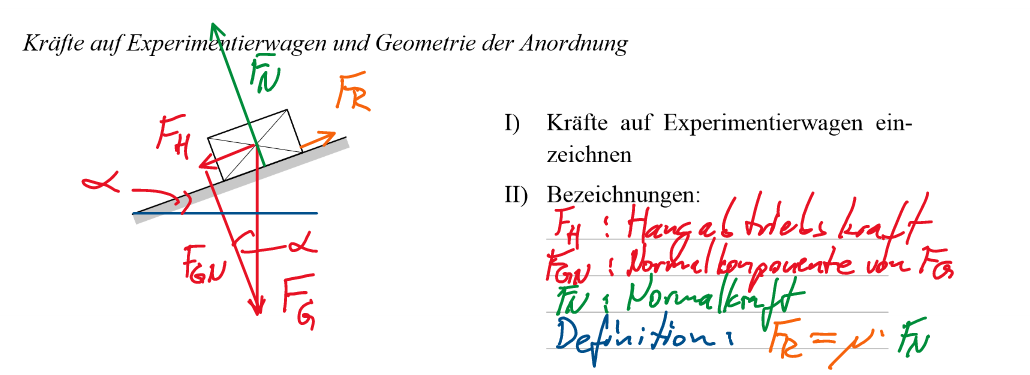
\includegraphics[width=\textwidth]{images/dynamik_schiefe_bahn.png}
  \begin{equation}
    F_R = \mu \cdot F_N
  \end{equation}
  \begin{equation}
    F_H = F_G \cdot \sin{\alpha}
  \end{equation}
  \begin{equation}
    F_N = F_{GN} = F_{G} \cdot \cos{\alpha}
  \end{equation}
  Resultierende Kraft:
  \begin{align}
    F_a &= F_H - F_R \\
    F_a &= F_G \cdot (\sin{\alpha} - \mu \cdot \cos{\alpha})
  \end{align}
  Daraus folgt bei a = 0:
  \begin{equation}
    \mu = \tan{\alpha}
  \end{equation}
  \begin{equation}
    [F] = N = kg \cdot \frac{m}{s^2}
  \end{equation}

  \subsubsection{Dichte}
  \begin{equation}
    \rho = \frac{m}{V}
  \end{equation}

  \section{Taschenrechner}
  \subsection{Stunden zu Stunden, Minuten and Sekunden konvertieren}
  \begin{equation}
    Zeit \blacktriangleright \mbox{DMS}
  \end{equation}

  \section{Konstanten}
  \begin{equation}
    g = 9.81 \si{\metre\per\square\second}
  \end{equation}
\end{document}